\documentclass[UserManual.tex]{subfiles}
\begin{document}
\setcounter{section}{1}

\section{Installation and Getting Started}\label{sec:installation}

\subsection{Prerequisites}
{\it Smooth Emulator} programs should run on UNIX, Mac OS or Linux, but is not supported for Windows OS. The software is largely  written in C++, though there are some python scripts included for graphing results. In addition to a C++ compiler (CMake files assume you can accommodate the  C++ 20 standard), the user needs the following software installed.

\begin{itemize}
    \item git
    \item CMake
    \item Eigen3 (Linear Algebra Package)
    \item Python/Matplotlib (only for generating plots)
\end{itemize}

CMake is an open-source, cross-platform build system that helps automate the process of compiling and linking for software projects. Hopefully, CMake will perform the needed gymnastics to find the Eigen3 installation. To install CMake, either visit the CMake website (https://cmake.org/), or use the system's package manager for the specific system. For example, on Mac OS, if one uses {\it homebrew} as a package manager, the command is
{\tt 
\begin{verbatim} % brew install cmake\end{verbatim}
}

Eigen is a C++ template library for vector and matrix math, i.e. linear algebra. The user can visit the Eigen website (\url{https://eigen.tuxfamily.org/dox/}), or use their system's package manager. For example on Mac OS with {\it homebrew},
{\tt 
\begin{verbatim} % brew install eigen\end{verbatim}
}

\subsection{Downloading the Repository and Copying Files to Working Directories}

The software requires downloading the BAND framework software repository into some directory. Should that be in the User's home directory, the User might enter
{\tt 
\begin{verbatim}
    /Users/CarlosSmith% git clone https://github.com/bandframework/bandframework.git
\end{verbatim}
}
Within the repository, there will be a directory\\{\tt /Users/CarlosSmith/bandframework/software/SmoothEmulator/}. All the relevant functionality of {\it Smooth Emulator} is contained within this directory. Throughout the manual the phrase {\tt \$\{GITHOME\_BAND\_SMOOTH\}} will refer to this directory. 

The User should create a personal directory from which the User would perform most projects. This is easiest accomplished by copying the template directory from the {\it Smooth} distribution. For example
{\tt
\begin{verbatim}
    % cp -r ${GITHOME_BAND_SMOOTH}/templates /Users/CarlosSmith/smoothy
\end{verbatim}
}
The User may choose any other name besides {\tt smoothy}. The directory {\tt ../smoothy/..} is the root directory for the User's executables and analyses data, and should be outside the {\tt bandframework/} path so that the User's work does not interfere with the repository. Within this directory one will find a template analysis directory, which is named  {\tt /Users/CarlosSmith/smoothy/analysis\_template}. One can copy that directory to a new directory, e.g. {\tt ../smoothy/my\_analysis}.
Hence forth, {\tt \$\{MY\_ANALYIS\}} is a name chosen by the User, and will refer to this directory, including the path, from which the User will perform most of the analysis. Thus, the User may wish to have several such directories, located according to the User's preference. Any time a new analysis is performed with new parameters, and if the User wishes to save the previous analysis, a new {\tt \$\{MY\_ANALYSIS\}} directory should be created. 

Within the {\tt smoothy/} directory, there is also a directory {\tt ../smoothy/mylocal/}, which after the copying above will become: {\tt /Users/CarlosSmith/smoothy/mylocal}. Henceforth, {\tt\$\{MY\_LOCAL\}} will refer to this directory, including its path. {\tt\$\{MY\_LOCAL\}/software/} contains the source code and CMake files for compiling the main programs. Executables will be stored in {\tt\$\{MY\_LOCAL\}/bin/}. Because the User might wish to edit the main programs, or to add similar programs, this provides the User a space to make such edits, all while leaving an original copy of the directory in the {\tt templates/} directory. The User may find it convenient to add {\tt \$\{MY\_LOCAL\}/bin/} to their path.


The philosophy behind this structure is that it allows the User to devise and build simple programs making calls to {\it Smooth Emulator} libraries without altering the source code and libraries which are kept in the {\tt \$\{GITHOME\_BAND\_SMOOTH\}/} directory structure. If the User wished to make modifications to this code, it would make sense to copy the {\tt \$\{GITHOME\_BAND\_SMOOTH\}/} directory to a new location. 

\begin{figure}[t]
\centerline{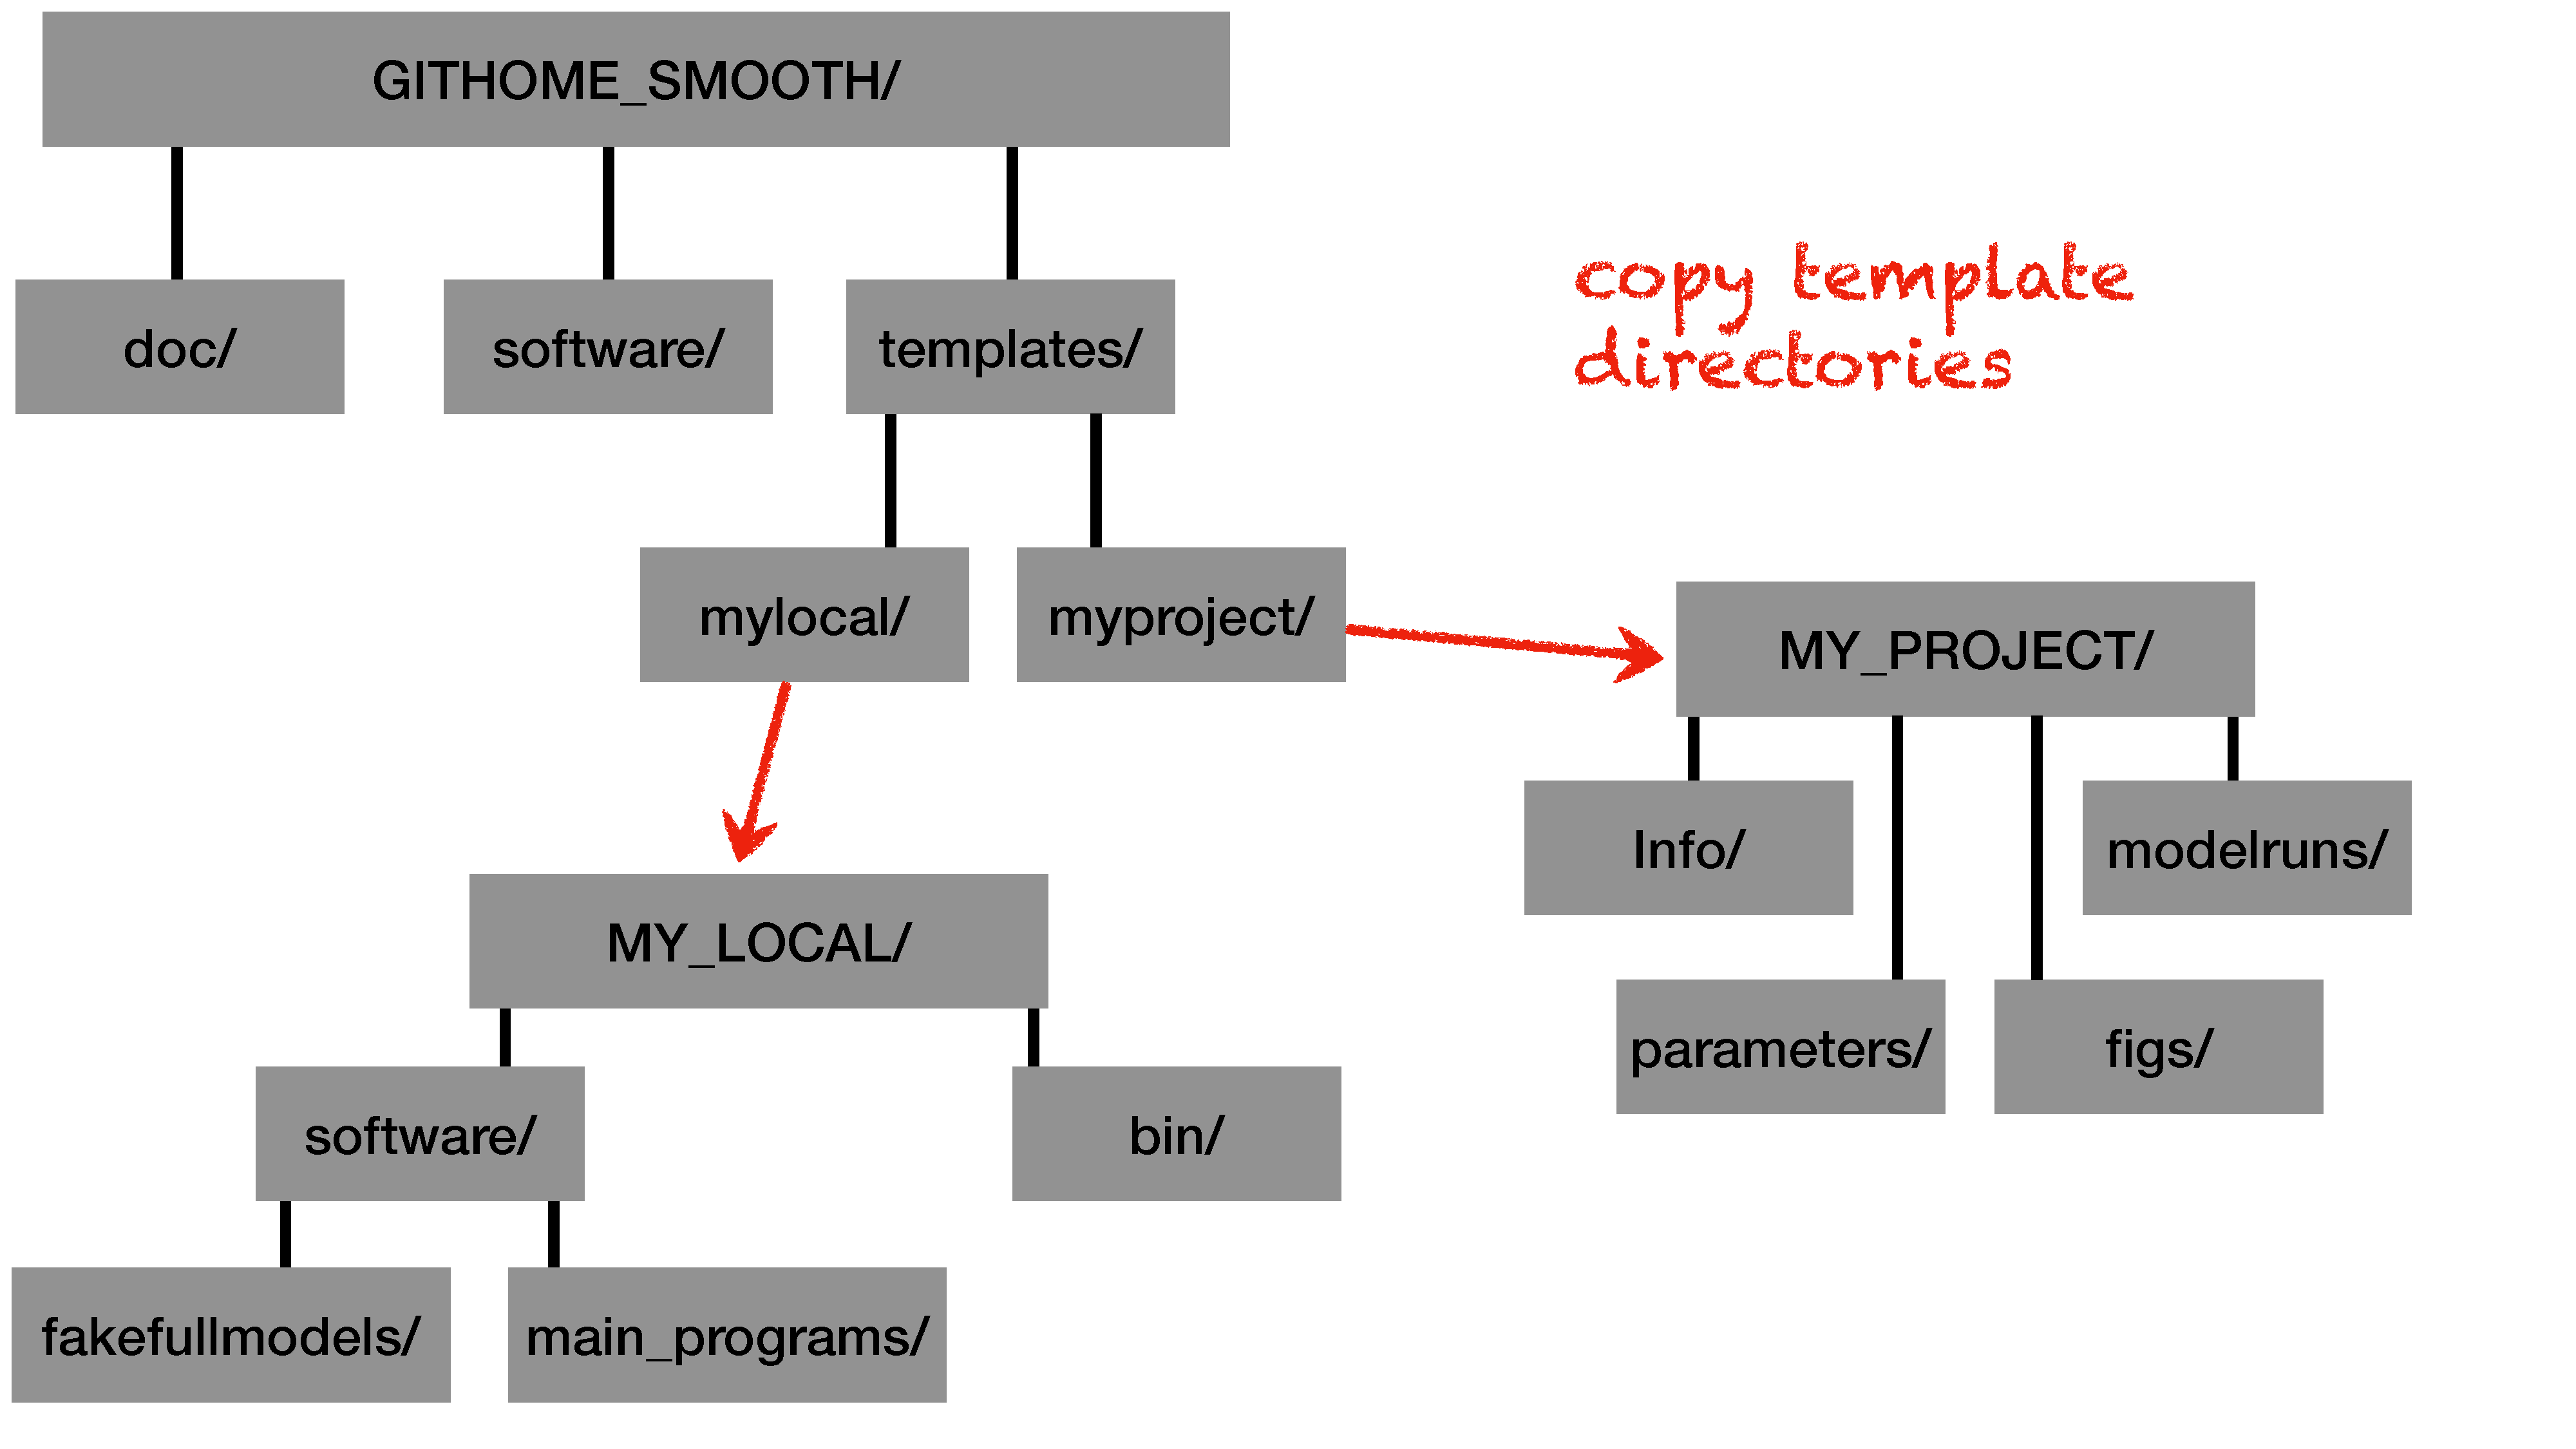
\includegraphics[width = 0.65\textwidth]{figs/directorystructure}}
\caption{\label{fig:directorystructure}{\bf The directory structure}: The User clones the repository into some location, which will be referred to as {\tt \$\{\tt GITHOME\_BAND\_SMOOTH\}}. From the {\tt templates} directory, the User copies the {\tt mylocal} and {\tt myanalysis} directories to two new locations, {\tt \$\{MY\_LOCAL\}} and {\tt \$\{MY\_ANALYSIS\}}. The User will likely make multiple copies of the {\tt myanalysis} directory for different projects or for different analyses with different options. The main source code and compiled libraries will be built and kept within the {\tt \$\{GITHOME\_SMOOTH\}/} tree. Source code for simple main programs can be found in {\tt \$\{MY\_LOCAL\}/software/} and executables are stored in {\tt \$\{MY\_LOCAL\}/bin/}. The software is designed to be run from the command line in the {\tt \$\{MY\_ANALYSIS\}} directory. Data used and created by {\it Smooth Emulator} software is stored in {\tt \$\{MY\_ANALYSIS\}/smooth\_data/}. 
}
\end{figure}

The directory structure is Fig. \ref{fig:directorystructure}. As stated above, for the remainder of this manual, {\tt \$\{GITHOME\_BAND\_SMOOTH\}/}, {\tt \$\{MY\_LOCAL\}/} and {\tt \$\{MY\_ANALYSIS\}/} will be used to denote the location of these directories. 

\subsection{Compiling the Software}

First, change into software directories, then create the makefiles with cmake, then compile them.
{\tt 
\begin{verbatim}
    % cd ${GITHOME_BAND_SMOOTH}/software
    % ${GITHOME_BAND_SMOOTH}/software% cmake .
    % ${GITHOME_BAND_SMOOTH}/software% make
\end{verbatim}
}
There seems to be a common problem that {\tt cmake} misreports the path of the {\tt Eigen} installation. If the User should get an error stating that the Eigen header files cannot be found, the User can set the environmental variable,
{\tt 
\begin{verbatim}
    % export EIGEN3_INCLUDE_DIR=/usr/local/include/eigen3
\end{verbatim}
}
The final arguments may need to be changed depending on the User's location of the packages. If the User wishes to choose a specific C++ compiler, the {\tt cmake} command should be replaced with {\tt cmake -D CMAKE\_CXX\_COMPILER=g++-11}, or whichever compiler is preferred. 

At this point all the libraries are built, but this does not include the main programs. The main programs are short, and are meant to serve as examples which the User might copy and edit at will. Before compiling, one needs to set an environmental variable so that the compilation can find the libraries needed for compilation.
{\tt
\begin{verbatim}
  % export GITHOME_BAND_SMOOTH=/Users/CarlosSmith/bandframework/software/SmoothEmulator
\end{verbatim}
}
The first part of the path needs to be replaced with the location of the {\tt bandframework} git repository. If one prefers not to set an environmental variable, one can instead edit\\
{\tt \$\{MY\_LOCAL\}/software/CMakeLists.txt}, and replace the line where the variable {\tt \$\{GITHOME\_BAND\_SMOOTH\}} is set to the shell's environmental variable with one where it is set explicitly.

Below, this illustrates how to compile the programs used for generating training points with Simplex and for tuning the emulator with {\it Smooth Emulator}:
{\tt
\begin{verbatim}
    % cd ${MY_LOCAL}/software
    % ${MY_LOCAL}/software% cmake .
    % ${MY_LOCAL}/software% make
    .
    .
\end{verbatim}
}
The {\tt cmake} command will also recompile the main libraries in {\tt \$\{GITHOME\_BAND\_SMOOTH\}/software/} if necessary. Several source codes for main programs can be found in\\
{\tt \$\{MY\_LOCAL\}/software/main\_programs/}. If you build your own main programs (probably using these as examples), you can edit the {\tt CMakeList.txt} file in {\tt \$\{MY\_LOCAL\}/software/main\_programs/}, using the existing entries as an example. The executables should appear in {\tt \$\{MY\_LOCAL\}/bin/}. 

\subsection{The \$\{{\tt MY\_ANALYSIS/smooth\_data}\} Directory}

Within {\tt \$\{MY\_ANALYSIS\}/smooth\_data} there are several sub-directories (assuming it was created from the template). The first is {\tt smooth\_data/Info/}. Information about the model parameters, and their priors is stored in {\tt smooth\_data/Info/prior\_info.txt}, and information about the observables is stored in {\tt smooth\_data/Info/observable\_info.txt}. The file {\tt smooth\_data/Info/experimental\_info.txt} stores information about the measurements for each observable, and is not needed for building the emulator, but is used by the MCMC investigation of the posterior. The {\tt smooth\_data/Options/} directory stores text files used to set options for the training-point optimization, the emulator and the MCMC programs. The {\tt smooth\_data/FullModelRuns} data has subdirectories {\tt run0/}, {\tt run1/} $\cdots$. Each subdirectory stores information describing a full model run. The file {\tt smooth\_data/FullModelRuns/runX/model\_parameters.txt} stores the model parameters used for run ``{\tt X}''. This file can be provided by the User, or it can be created by the training-point optimization codes. Once those files are created, it is the User's responsibility to run the full model and record the observables in {\tt smooth\_data/FullModelRuns/runX/obs.txt}. Given those observables, the User can then run the emulator software. If the User runs the MCMC software, the MCMC traces are stored as text files in {\tt smooth\_data/MCMC\_Trace/}. Examples of PYTHON scripts for graphing using MATPLOTLIB can be found in {\tt smooth\_data/figs/}.

\end{document}
